\documentclass[notitlepage, 12pt, a4paper, twoside, titlepage]{article}
\usepackage{graphicx}
\usepackage[left=1in, right=1in, top=1in, bottom=1in]{geometry}

\usepackage{amsmath}
\usepackage{titling}
\usepackage{lipsum}

\pretitle{\begin{center}\Huge\bfseries}
\posttitle{\par\end{center}\vskip 0.5em}
\preauthor{\begin{center}\Large\ttfamily}
\postauthor{\end{center}}
\predate{\par\large\centering}
\postdate{\par}
\title{Statistical Data Analysis, Assignment 3}
\author{Roel Deckers  \\
	Utrecht University
	}

\date{\today}
\begin{document}
\maketitle

\section{Objective}
To test the {\em Central Limit Theorem (CLT)} as it applies to a Uniform distribution between 0 and 1, an exponential distribution $f(x) = \exp(-x)$, and the standard "Cauchy"\footnote{Technically the ratio distribution but we follow the definitions established by the assignment.} distribution.

\section{Theory}
The central limit theorem states that the mean of $N$ samples drawn from a distribution $D$ will converge to a normal distribution $D_N$ with mean $E\left[D_N\right] = E\left[D\right]$ and variance $var(D_N) = var(D)/N$ for large $N$, {\em if} $D$ has well defined moments.
\par The uniform distribution is well defined with mean $0.5$ and a standard deviation of $1/12$. The exponential distribution is well defined with both a mean an a standard deviation of $1$, and the Cauchy distribution has no
well defined mean or standard deviation.

\section{The Distributions}
Using the ROOT framework we generated our three distributions and plotted them in figure \ref{fig:dist}. We let ROOT compute the mean and standard deviations of our binned histograms, as shown in the top right of each graph, and we also computed it
over our raw data. The results of these computations are given in table \ref{tbl:mean}. \par Note how the uniform and exponential distribution are in close agreement (with minor differences attributable to the binning procedure) but the Cauchy distribution produces wildly different results.
We believe this can be attributed to a combination of the ill-defined variance of the Cauchy Distribution and the binning procedure removing all outliers.

\begin{table}[h!]
\centering
\begin{tabular}{|l||l|}
\hline
{\bf Distribution} & \bf{mean}\\
\hline
normal & $0.5 \pm 0.3$ \\ \hline
exponential & $1 \pm 1$ \\ \hline
Cauchy & $0 \pm 2\times 10 ^2$ \\ \hline
\end{tabular}
\caption{Mean and standard deviation for (unbinned) distributions with $N=1$.}
\label{tbl:mean}
\end{table}

\begin{figure}[h!]
  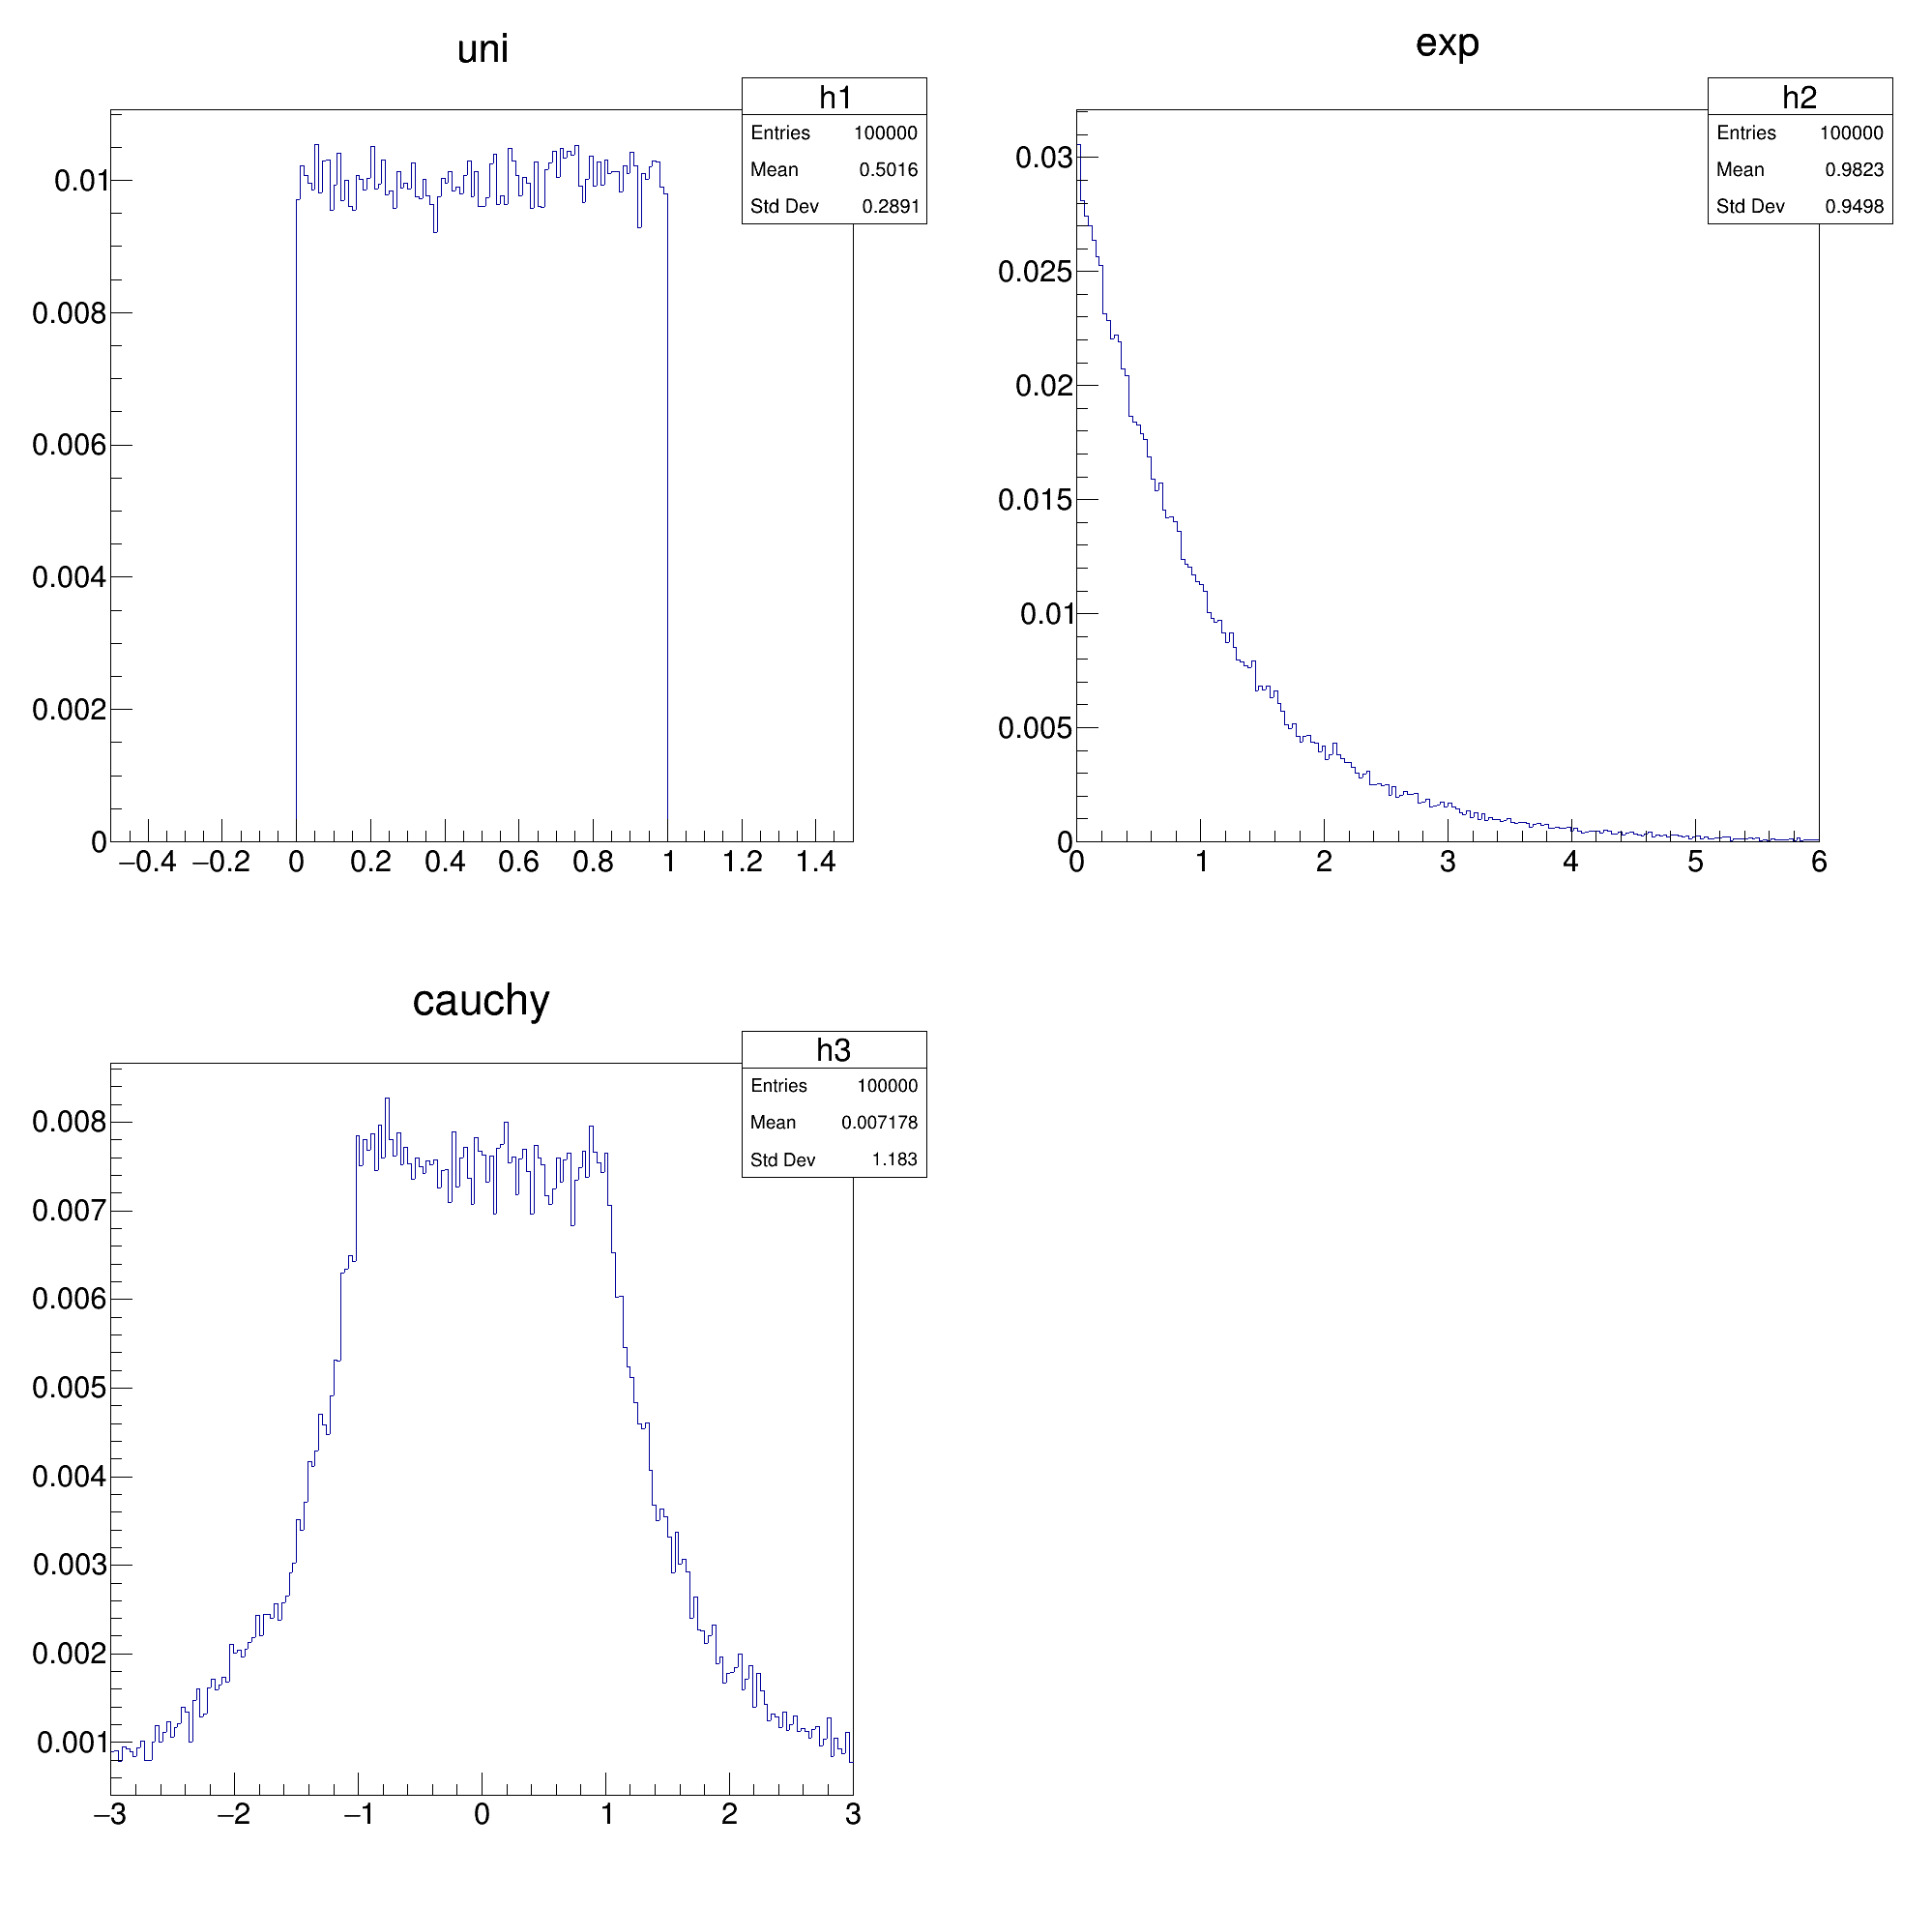
\includegraphics[width=\linewidth]{../distributions.png}
  \caption{Our base distributions $D$.}
  \label{fig:dist}
\end{figure}

\section{Distributions for $N$ samples}
Subsequently we plotted the distributions of the mean of $N$ samples from each distribution, for multiple $N$, in figure \ref{fig:dist2}. We see that, as expected, the uniform and exponential distribution converge to a sharply peaked normal distribution as we average more samples.
The Cauchy distribution however does not show much difference between $N = 10$ or $N = 100$ and if one looks closely does not resemble a normal distribution at all: the tail-ends are flared too much for a normal distribution.

\begin{figure}[h!]
  \includegraphics[width=\linewidth]{../dist2.png}
  \caption{$D_N$ for various $D$ and $N$.}
  \label{fig:dist2}
\end{figure}

\section{Mean and variance}
The CLT predicts that as we increase $N$ the mean would remain unchanged, therefore we plotted the mean of the histograms (as computed by ROOT) against $N$ in figure \ref{fig:mean}. All of them seem to be stable, even the Cauchy distributions, this is reasonable because it is a symmetric distribution and any outliers
due to ill-defined variance will be dealt with by the binning process.
Furthermore, the CLT predicts that the standard deviation will go as $\sigma_{D_N} = \sigma_D/\sqrt{N}$, therefore the ratio $\sqrt{N}\sigma_{D_N}/\sigma_{D}$ should be equal to one if the CLT holds. We have plotted this ratio in figure \ref{fig:stddev} using the results in table \ref{tbl:mean} for $\sigma_D$\footnote{using the histogram computed value for $\sigma_D$ produces a small and fixed relative offset for uniform and exponential, but still produces wildly wrong results for Cauchy.}.

\begin{figure}[h!]
  \includegraphics[width=\linewidth]{../mean.png}
  \caption{Means of $D_N$ for various $D$ as a function of $N$.}
  \label{fig:mean}
\end{figure}

\begin{figure}[h!]
  \includegraphics[width=\linewidth]{../stddev.png}
  \caption{ $\sigma_{D_N} = \sigma_D/\sqrt{N}$ for various $D$ as function of $N$.}
  \label{fig:stddev}
\end{figure}

\section{Conclusion}
Unsurprisingly, the CLT holds. For uniform and exponential distributions it correctly predicts the results. For the Cauchy distribution it does not make any (correct) predictions, but this is in line with our expectations: the Cauchy distribution does not have well defined moments.


\end{document}
